\documentclass[a4paper,12pt,french]{article}
\usepackage[margin=2cm]{geometry}
\usepackage[thinfonts,latinmath]{uglix2}
\usepackage{colortbl,amssymb}
\pagestyle{empty}
\let\oldemptyset\emptyset
\let\emptyset\varnothing
\nouveaustyle
\begin{document}
\titreinterro{Interrogation}{SIO1}{03/2022}


\exo{}\\

$A=\left\lbrace a\,;\,b\,;\,c\,;\,d\right\rbrace$ et $B=\left\lbrace 1\,;\,2\,;\,3\right\rbrace$.
\begin{enumerate}[\bfseries 1.]
	\item 	Donner 3 éléments de $A\times B$.
	\item 	Combien d'éléments comporte $A\times B$ ?
    \item 	Combien d'éléments $\mathcal{P}(A\times B)$ possède-t-il ?\\
\end{enumerate}


\exo{}\\

On définit la relation $\mathcal{R}$ de la manière suivante :\\ deux entiers $x$ et $y$ vérifient $x\mathcal{R}y$ si et seulement si $x\neq y$.\\

Cette relation est-elle (justifier)
\begin{enumerate}[\bfseries 1.]
	\item 	réflexive ?
	\item 	symétrique ?
    \item 	antisymétrique ?
    \item 	transitive ?\\
\end{enumerate}
\exo{}\\

\begin{enumerate}[\bfseries 1.]
	\item 	Sur cette feuille, barrer un minimum de flèches pour que la relation soit antisymétrique.
            \begin{center}
            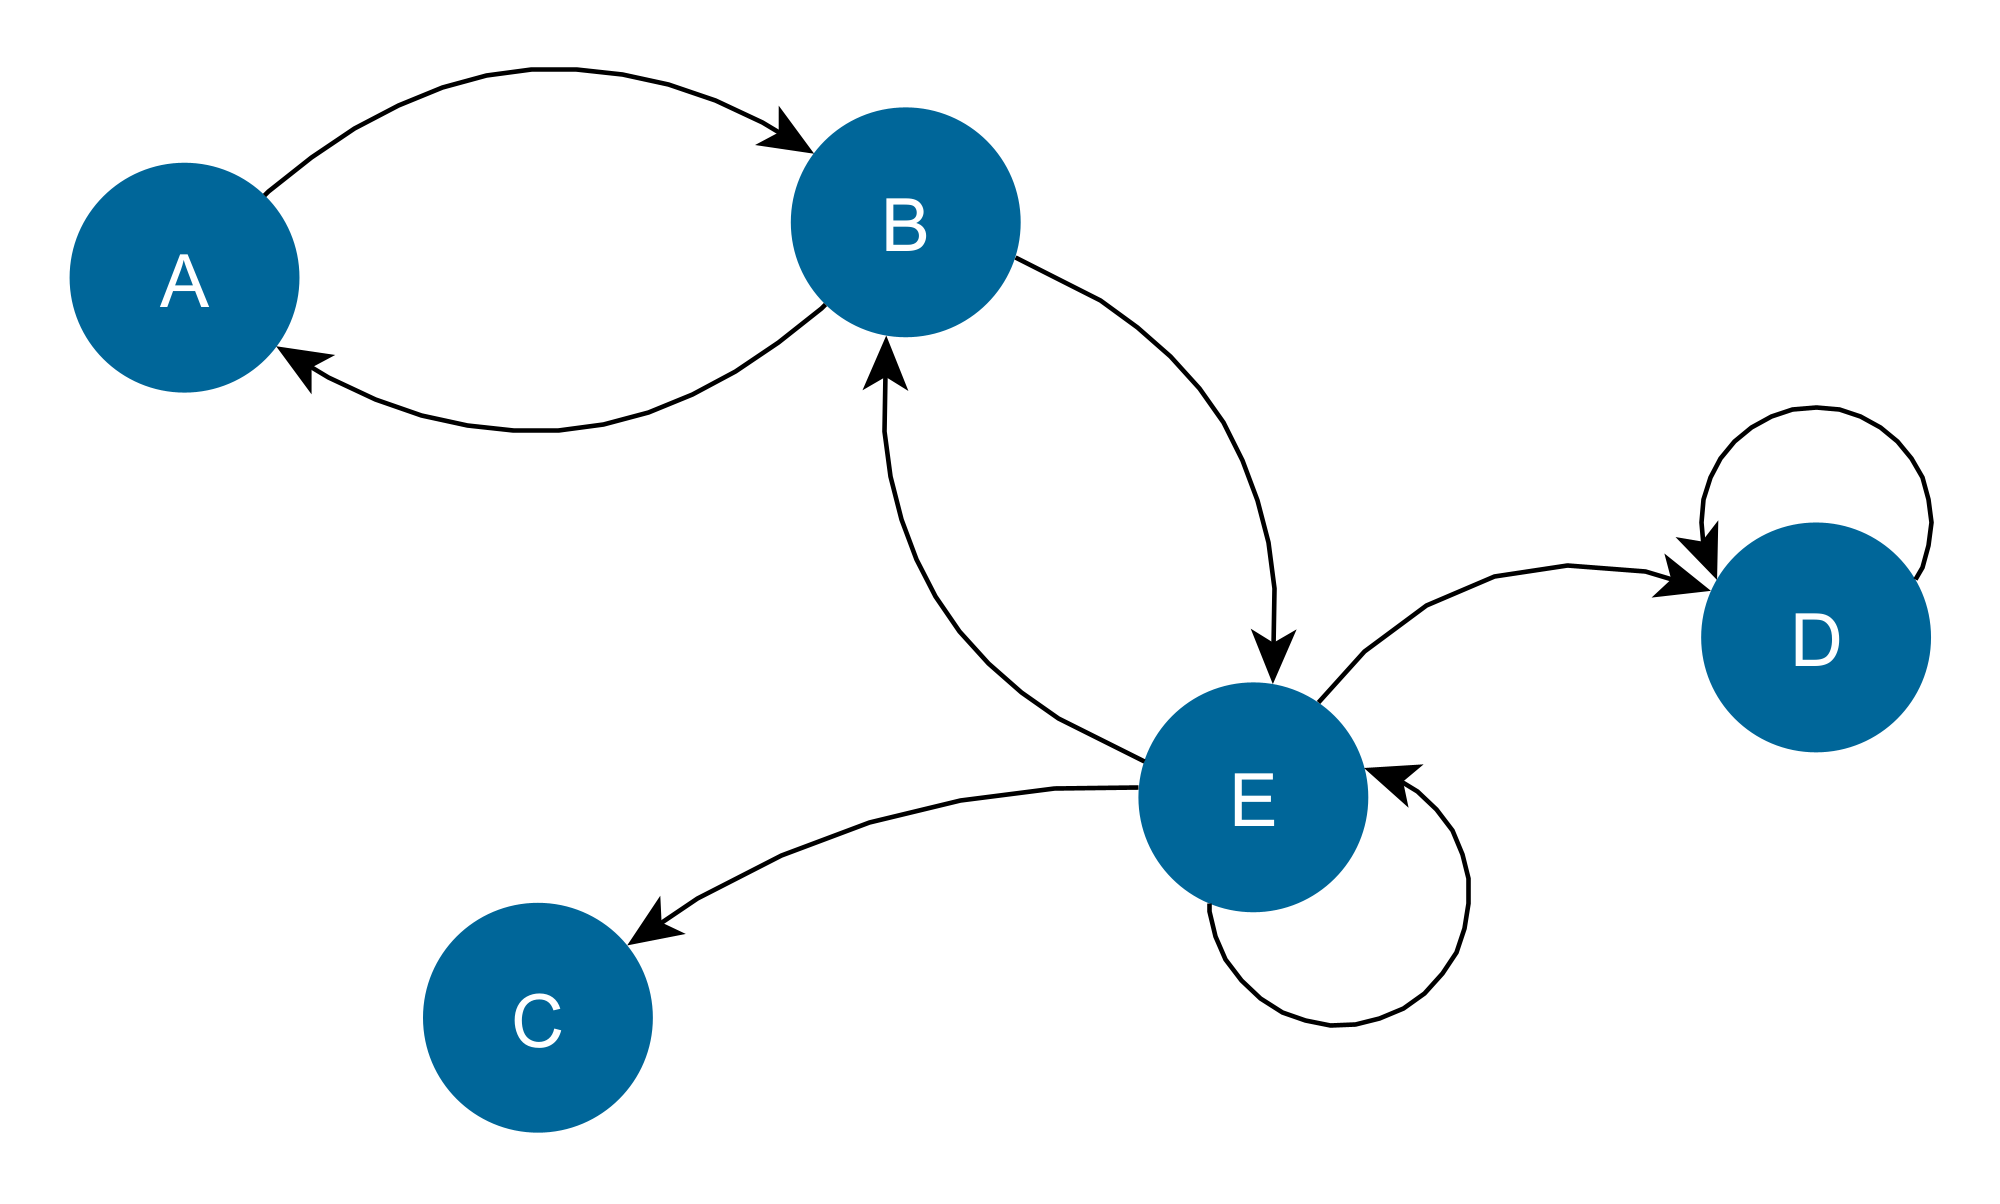
\includegraphics[width=7cm]{img/2antisym}
            \end{center}
	\item 	Sur cette feuille, ajouter un minimum de flèches pour que la relation soit transitive.
            \begin{center}
            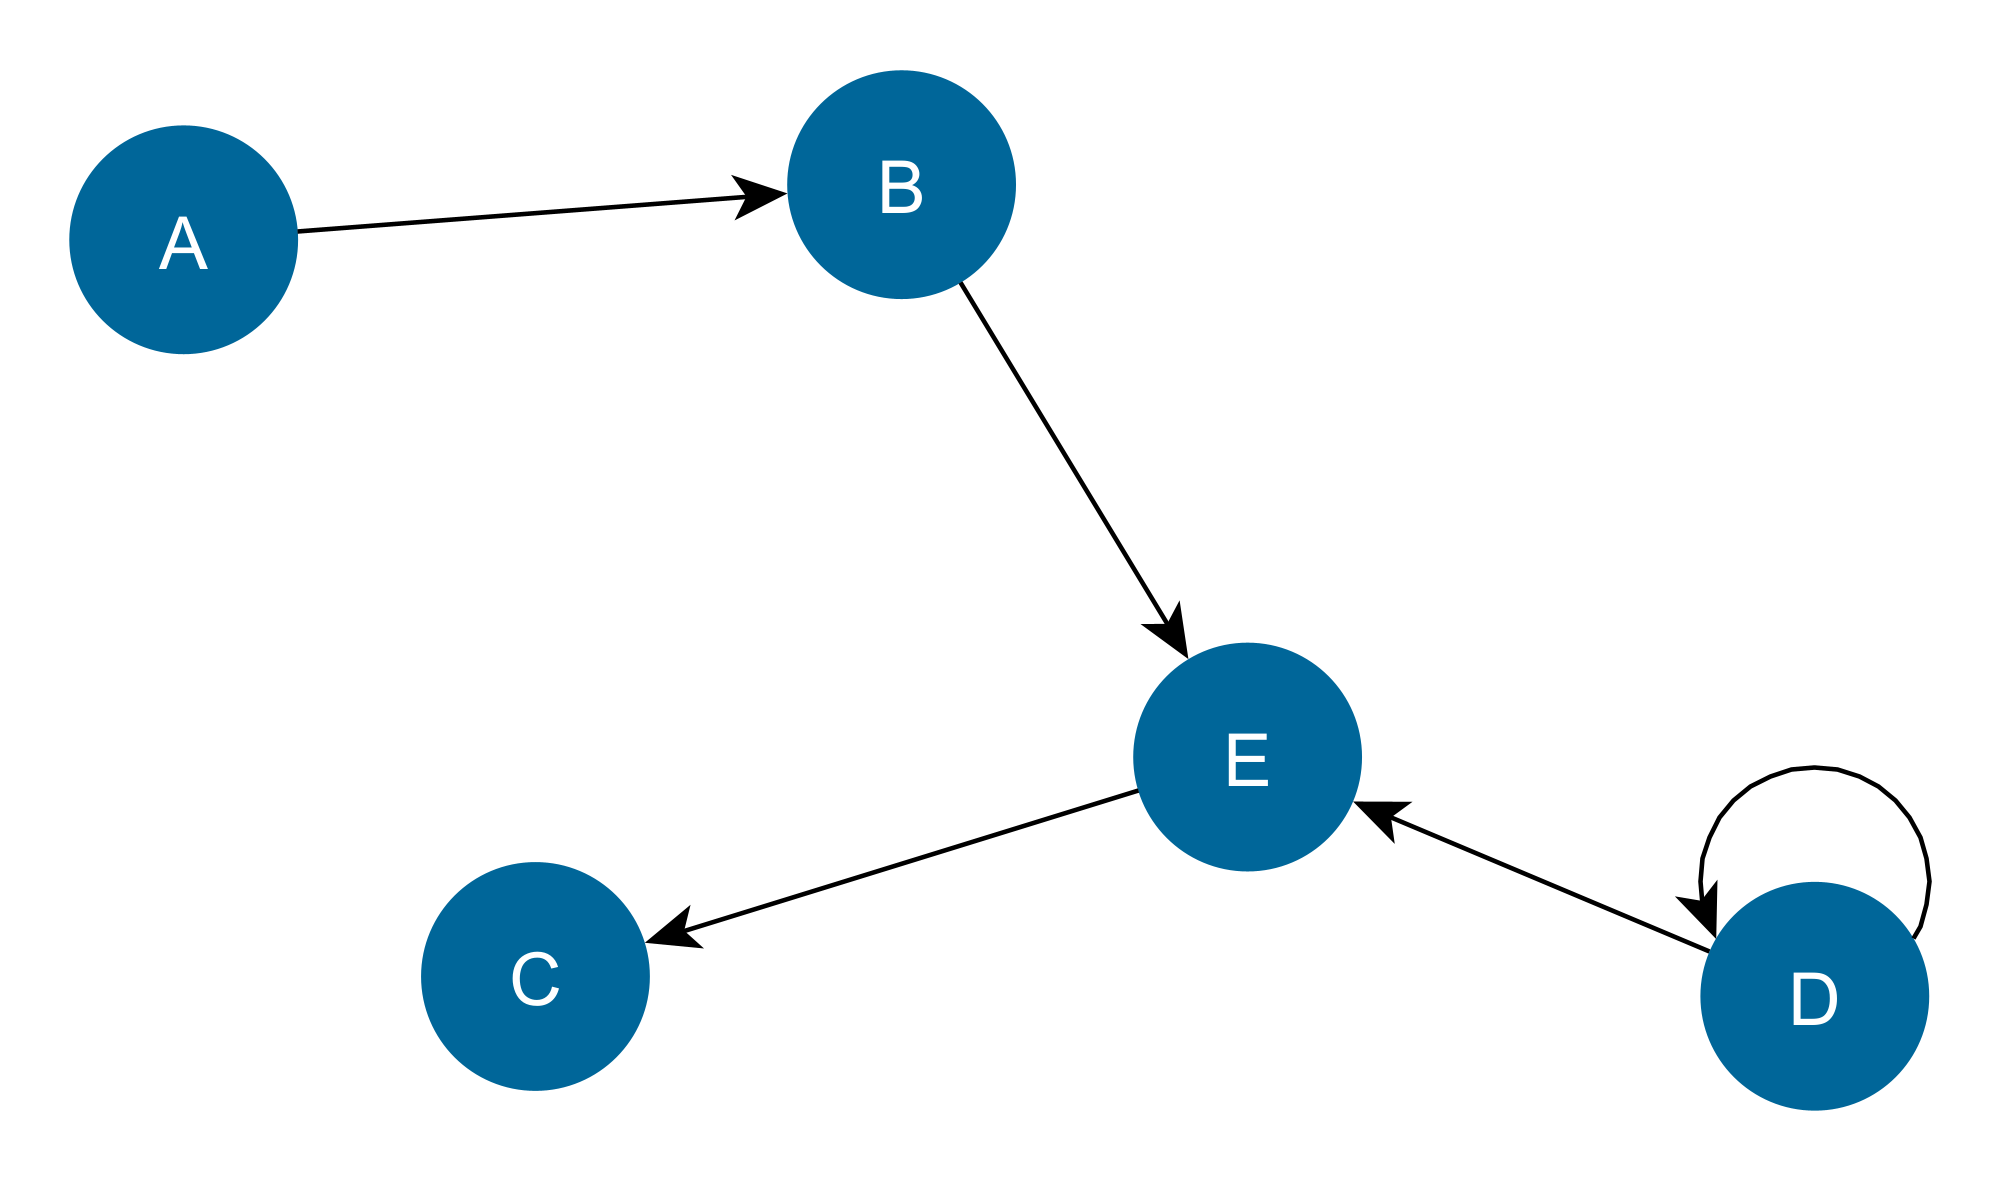
\includegraphics[width=7cm]{img/2trans}
            \end{center}
\end{enumerate}


\exo{}\\

$A$ et $B$ sont deux parties de $E$. Colorier l'ensemble demandé.
	\begin{multicols}{2}
    \begin{enumerate}[\bfseries 1.]
		\item 	$A\cap (B\cup C)$\\
                \begin{center}
                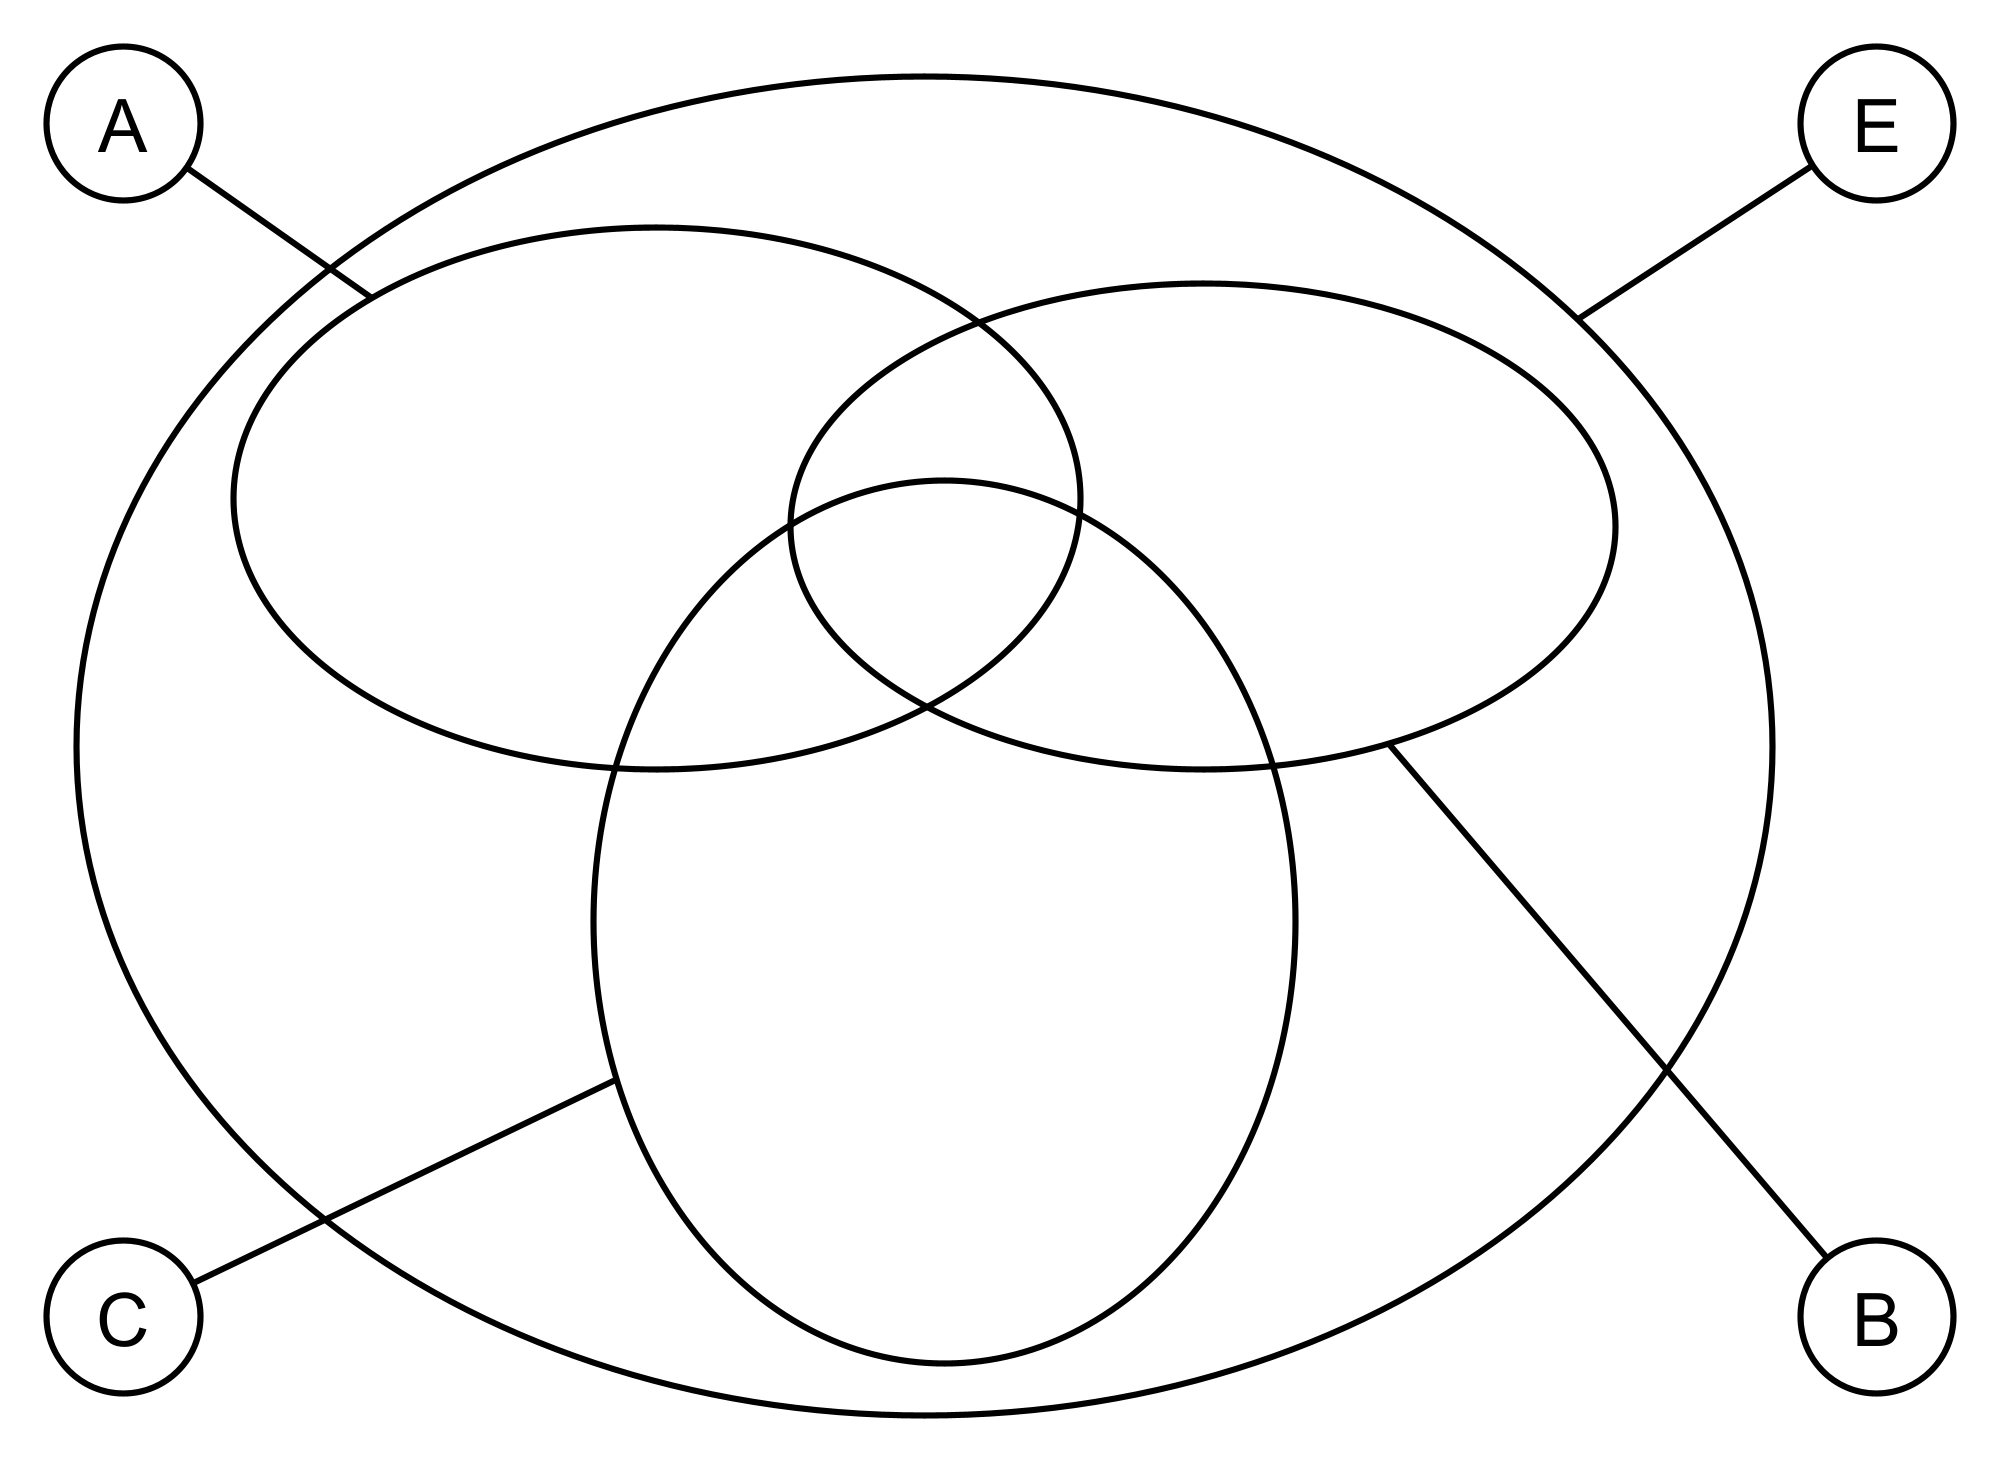
\includegraphics[width=4cm]{img/venn}
                \end{center}
		\item 	$(A\cap B)\cup C$\\
                \begin{center}
                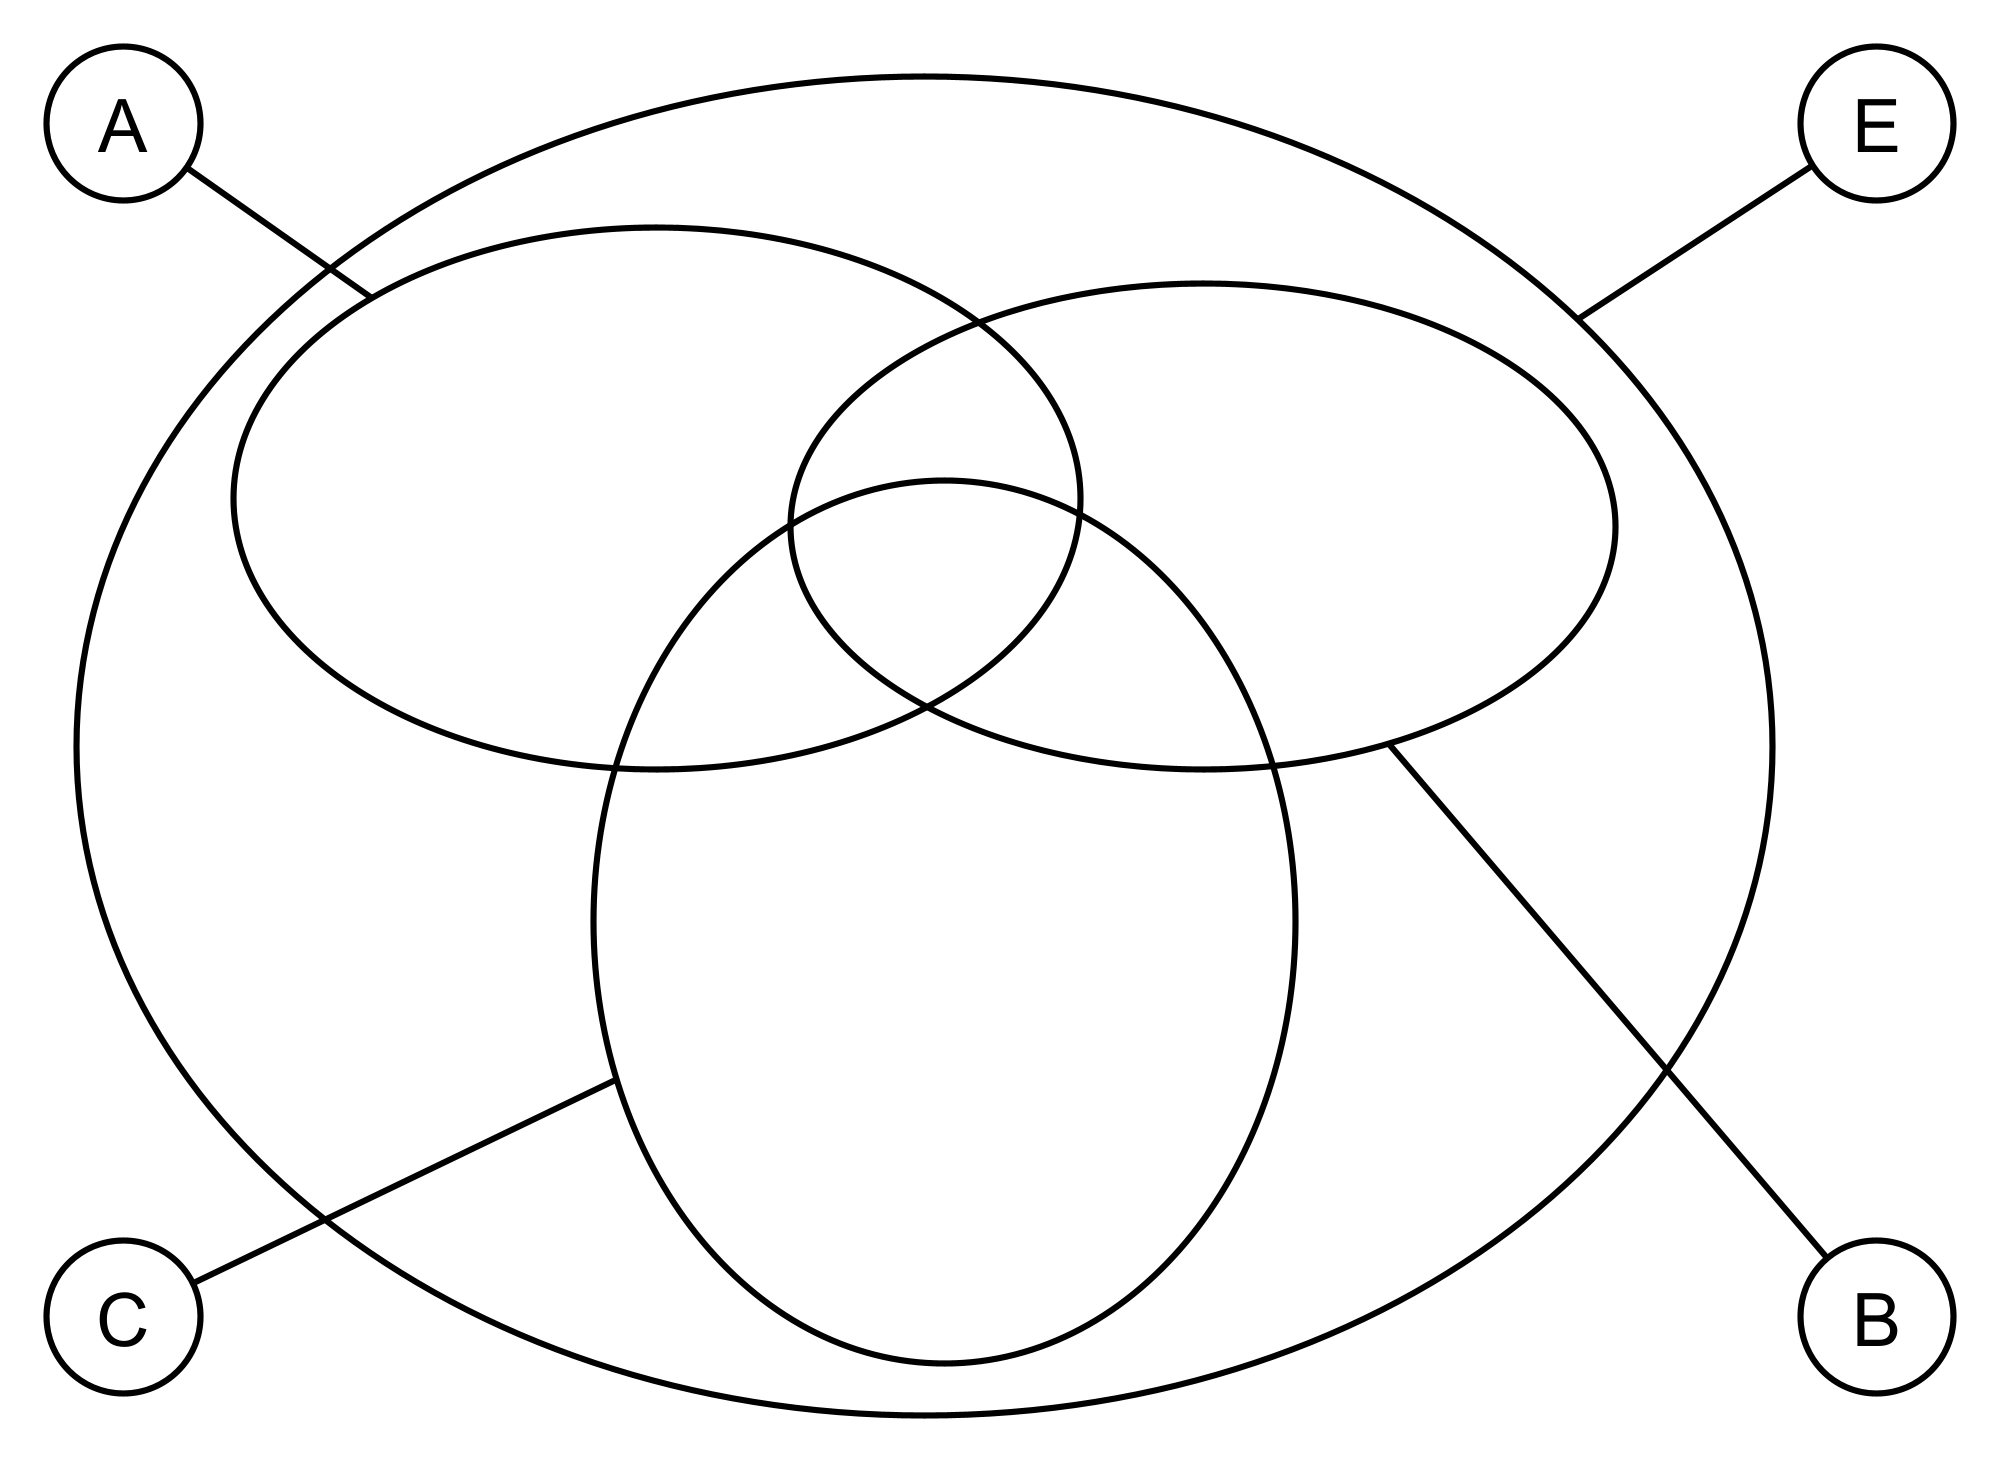
\includegraphics[width=4cm]{img/venn}
                \end{center}
		\item 	$A\cap B\cap \barmaj{C}$\\
                \begin{center}
                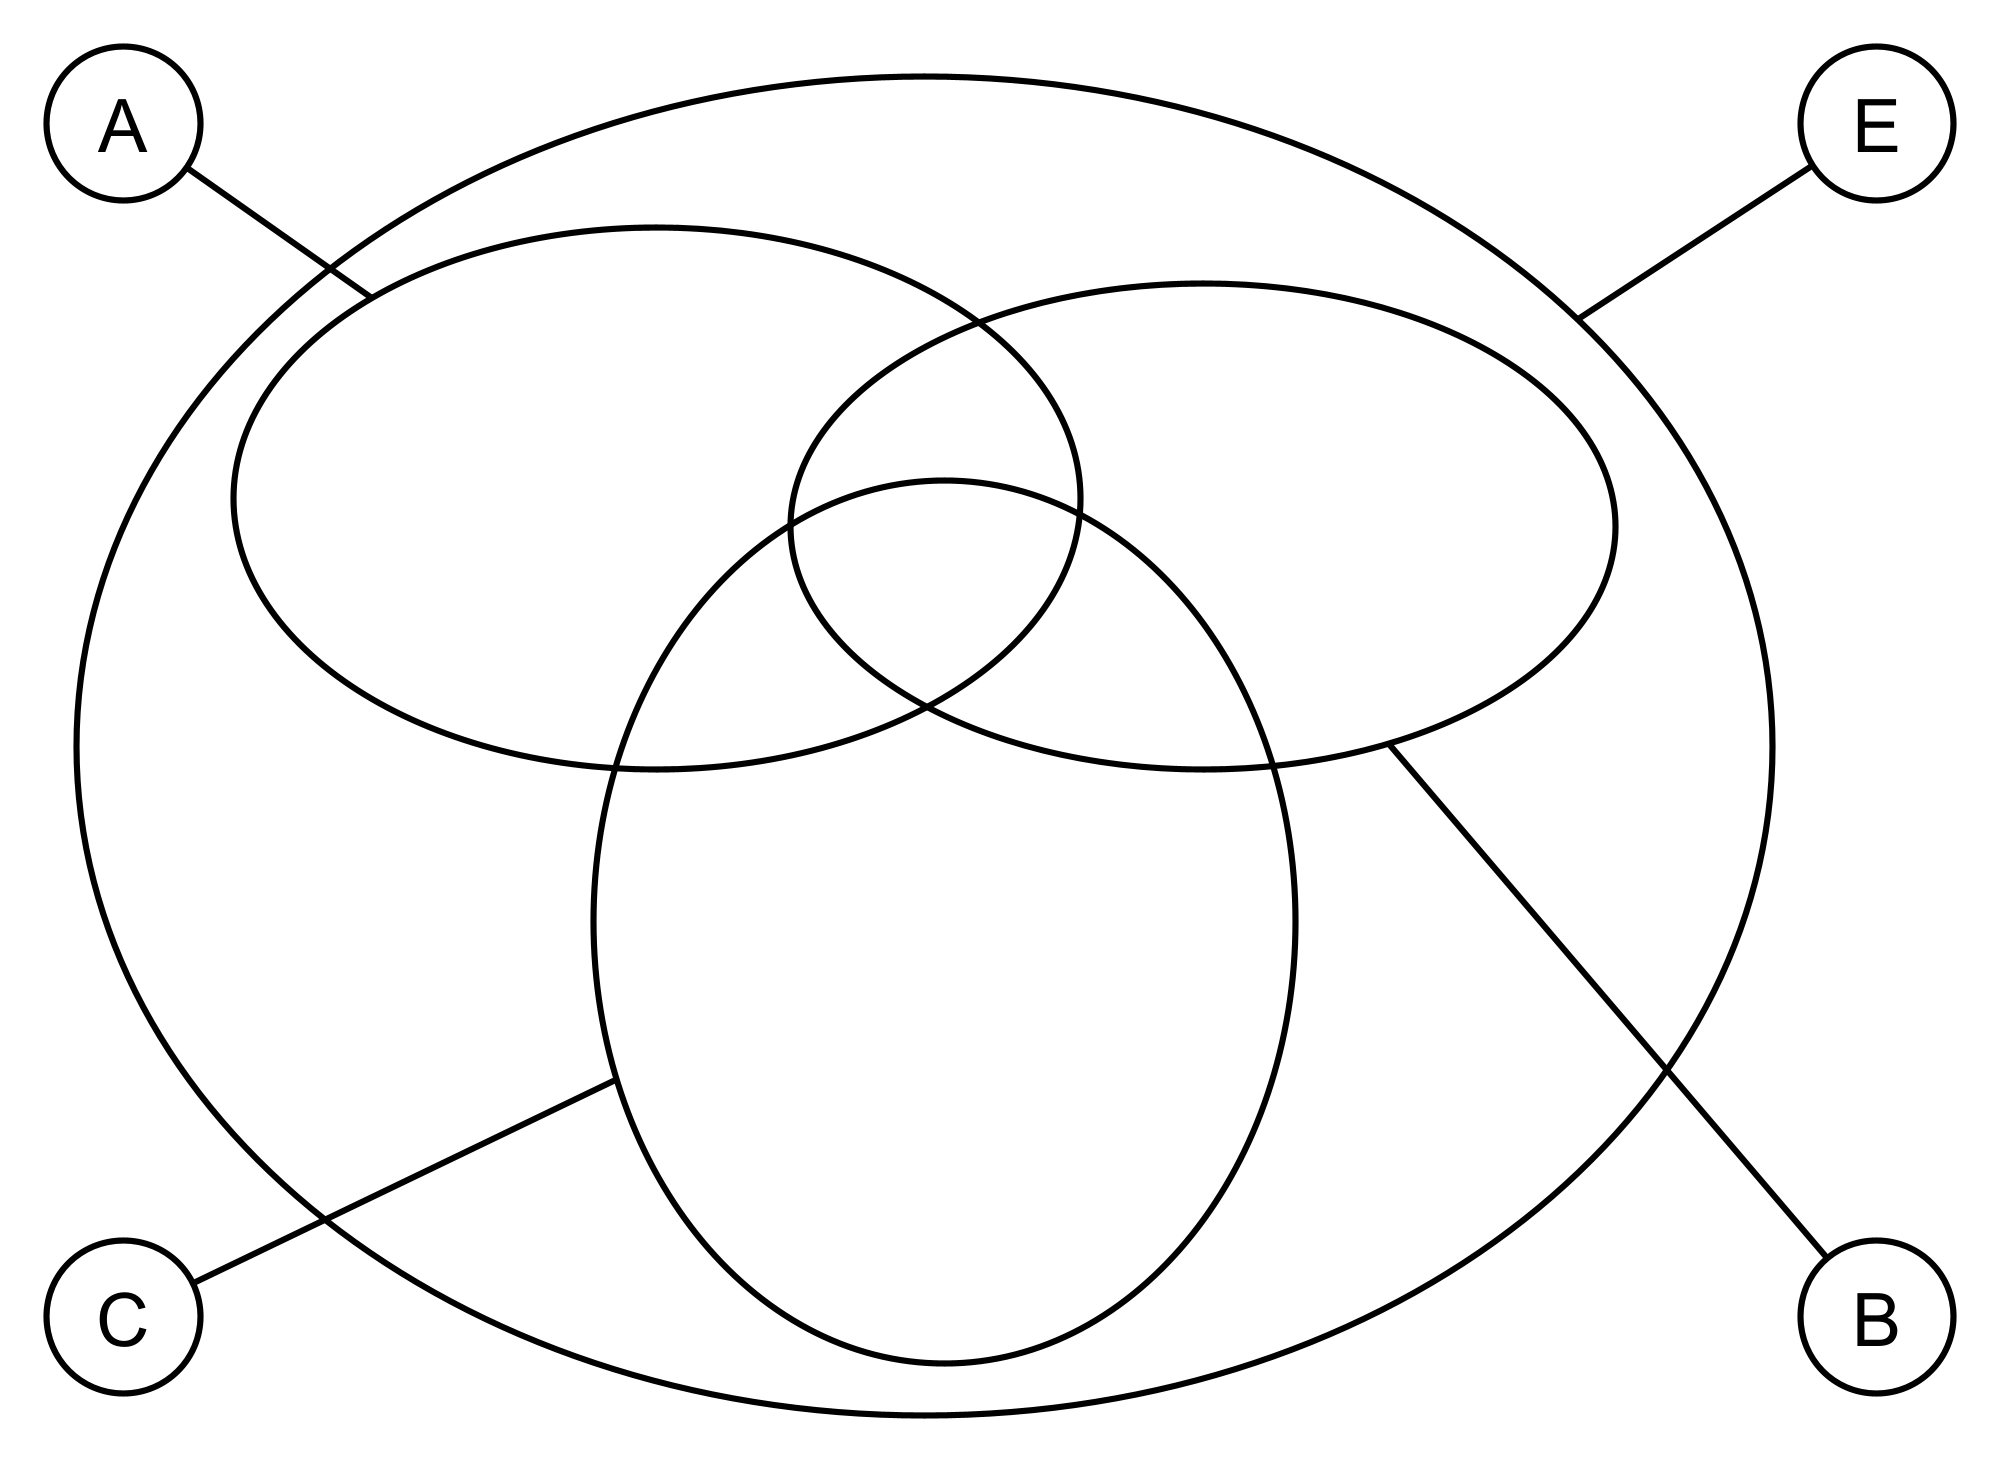
\includegraphics[width=4cm]{img/venn}
                \end{center}
		\item 	$\barmaj{A}\cup\barmaj{B}\cup\barmaj{C}$\\
                \begin{center}
                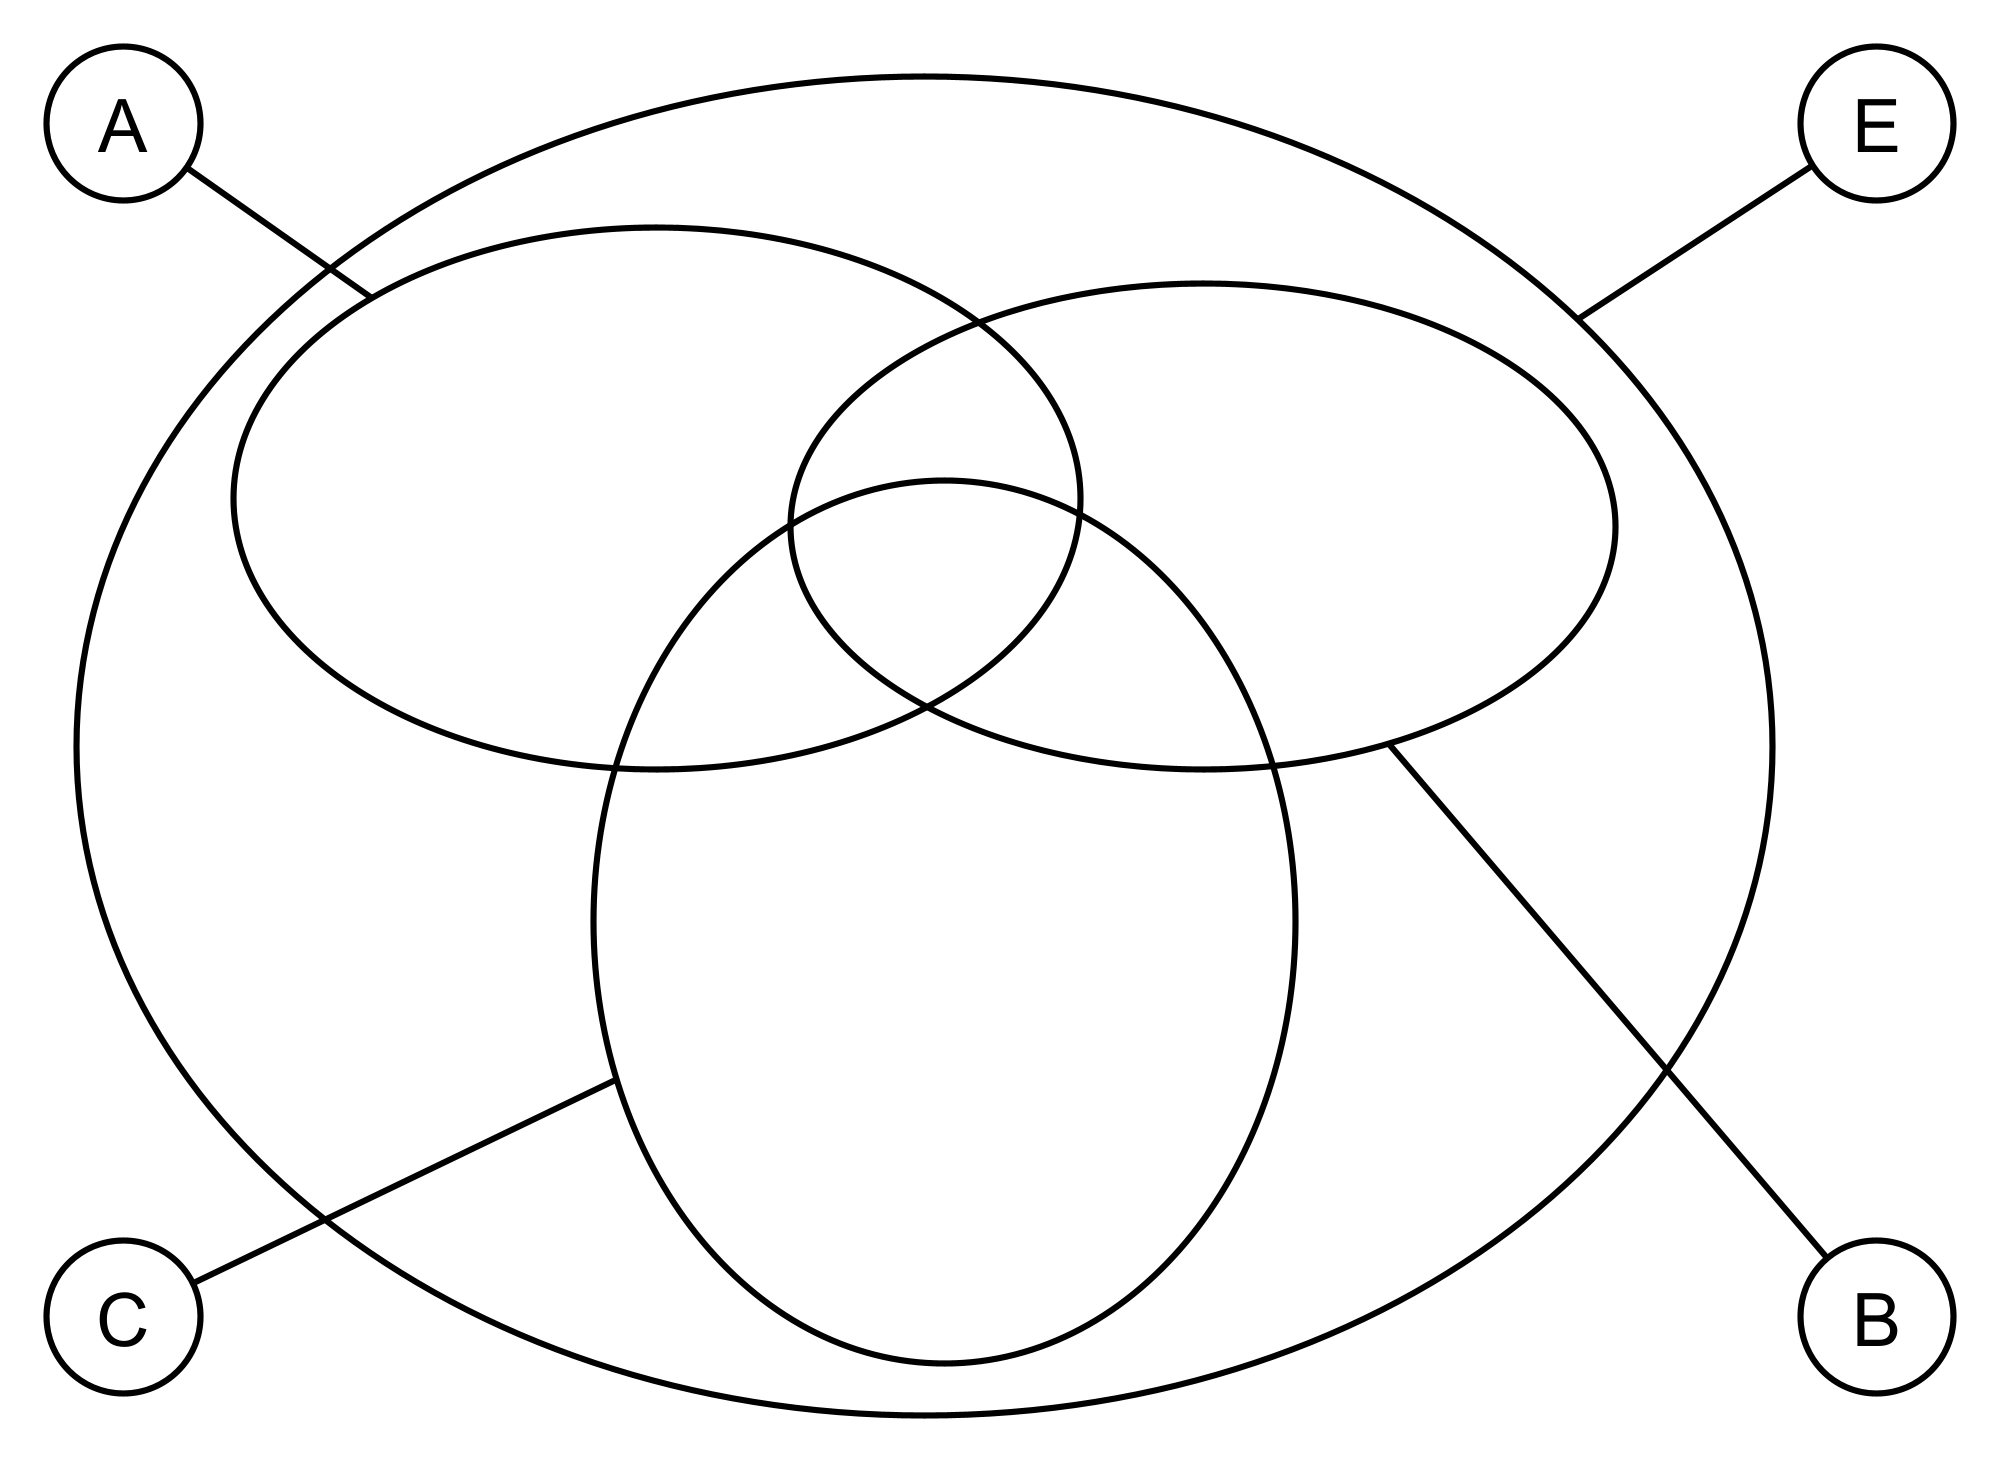
\includegraphics[width=4cm]{img/venn}
                \end{center}
		\end{enumerate}
	\end{multicols}

\exo{}\\

On considère $\mathcal{E}$ l'ensemble des \pythoninline{list} d'\pythoninline{int} en \textsc{Python}.\\
Ainsi \pythoninline{[1, 2]} est un exemple d'élément de $\mathcal{E}$.\\
Sur $\mathcal{E}$ on définit la relation $\preccurlyeq$ de la manière suivante :\\

\pythoninline{L1} $\preccurlyeq$ \pythoninline{L2} signifie qu'au moins une des deux conditions suivantes est vérifiée :
\begin{enumerate}[\textbullet]
	\item 	 \pythoninline{L1[0] <= L2[0]}
	\item 	\pythoninline{L1[0] == L2[0] and L1[1] <= L2[1]}	\\
\end{enumerate}

\begin{enumerate}[\bfseries 1.]
	\item 	Montrer que \pythoninline{[2, 7]} $\preccurlyeq$ \pythoninline{[4, 1]}.
	\item 	Montrer que \pythoninline{[2, 7]} $\preccurlyeq$ \pythoninline{[2, 9]}.
    \item 	Montrer qu'il existe une telle relation entre \pythoninline{[5, -7]} et \pythoninline{[1, -3]}.
    
    \item	Montrer que $\preccurlyeq$ est réflexive.
    \item 	Montrer que $\preccurlyeq$ est antisymétrique.
    \item 	Montrer que $\preccurlyeq$ est transitive.
    \item 	Que peut-on en déduire pour $\preccurlyeq$ ?
\end{enumerate}

\end{document}
